\chapter {Forecast}

The forecasting has been implemented in three differents ways: SARIMA , MLP and LSTM.
A subset of dataset has been used on forecast.This choice was made to avoid working on too many interpolated data; this also allowed us to reduce the training time for the forecasting models, particularly LSTM and MLP,
Indeed, the dataset is filtered on players that played more than 100 matches in the considered range of three years, resulting on 25 selected.
Fantavotes for each player have been divided into train and test sets (70\% - 30\% respectively).
Performance are compared in table \ref{table:RMSE} using \textit{Root Mean Squared Error} (RMSE) as common metric.

\section{SARIMA}

Regarding SARIMA, \textit{auto-arima} function has been used to find the best parameters for ARIMA model.
An example of application of SARIMA model is visible in Figure \ref{fig:sarima}

\begin{figure}[H]
  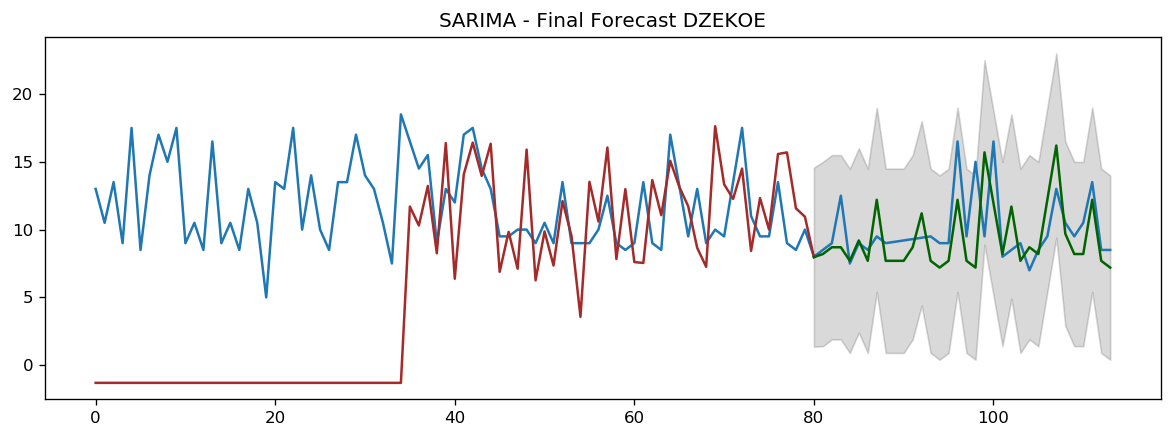
\includegraphics[scale=0.5]{images/dzeko_sarima_fantavoti.png}
   \centering  
   \caption{\textit{SARIMA forecast on ''Edin Dzeko''.}}
  \label{fig:sarima}
\end{figure}

\section{MLP}
The MLP model architecture includes 1 input layer with 12 nodes, 1 hidden layer with 38 nodes and 1 output layers with 1 node. The activation function is \textit{RELU}.
The network has been trained with \textit{Adam} optimizer and 150 epochs.
An example of application of the MLP model is visible in Figure \ref{fig:mlp}
\begin{figure}[H]
  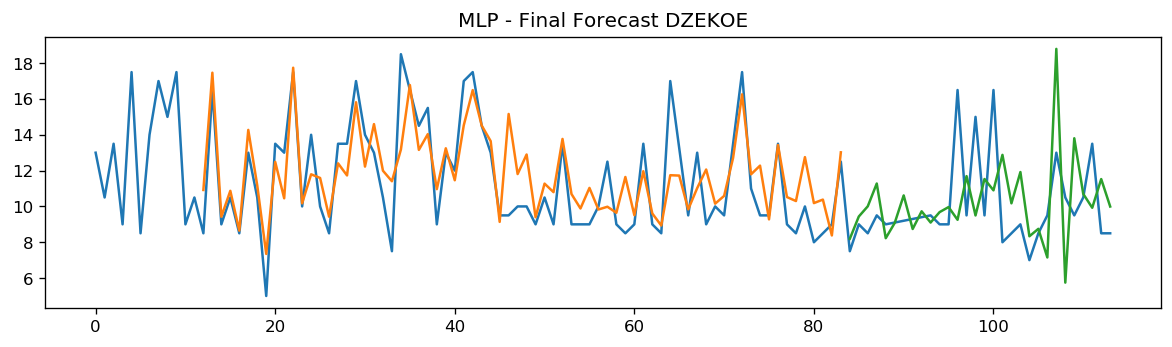
\includegraphics[scale=0.5]{images/dzeko_mlp_fantavoti.png}
   \centering  
   \caption{\textit{MLP forecast on ''Edin Dzeko''.}}
  \label{fig:mlp}
\end{figure}

\section{LSTM}
The LSTM architecture includes 1 input layer with 12 nodes, 1 hidden layer with 32 LSTM cells and 1 output layers with 1 node. The activation function is \textit{relu}.
The network has been trained with Adam optimizer and 75 epochs.
An example of application of the LSTM model is shown in Figure \ref{fig:mlp}
\begin{figure}[H]
  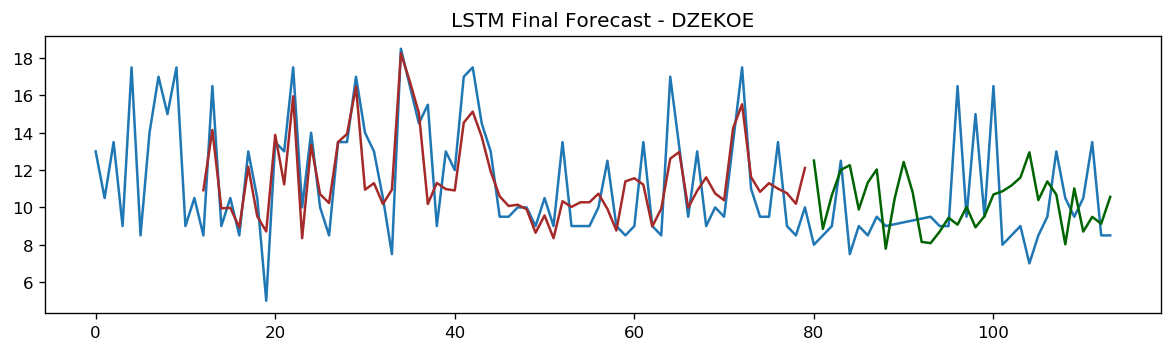
\includegraphics[scale=0.5]{images/dzeko_lstm_forecast.png}
   \centering  
   \caption{\textit{LSTM forecast on ''Edin Dzeko''.}}
  \label{fig:mlp}
\end{figure}


\section{Models combination}

In order to improve accuracy  on predictions, two type of models: statistic (SARIMA) and neural (LSTM)  were ensembled to come up with an hybrid version.

The final model used for forecasting is defined as:
\\
\begin{center}
  $\alpha * LSTM + (1 - \alpha) * SARIMA$
\end{center}
where:
\begin{itemize}
    \item \textbf{$\alpha$} is a weight in $[0; 1]$ that minimizes the RMSE 
    \item \textbf{LSTM} is the value predicted by LSTM model
    \item \textbf{SARIMA}  is the value predicted by SARIMA model 
\end{itemize}


\begin{figure}[H]
  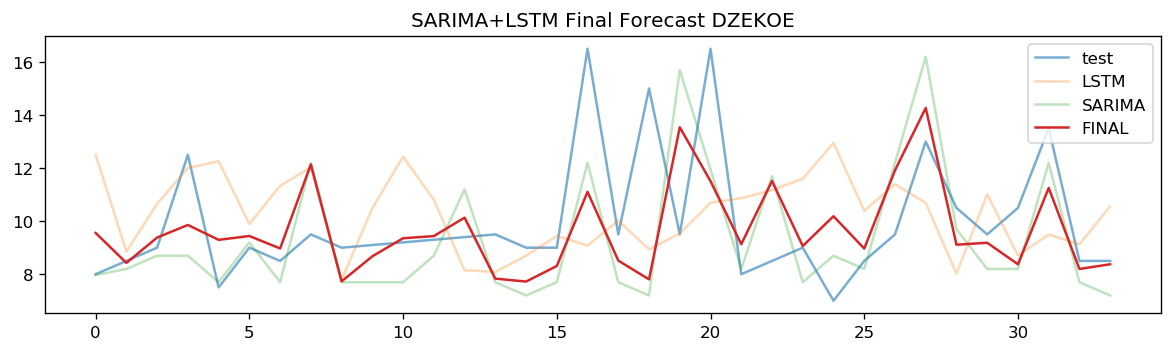
\includegraphics[scale=0.5]{images/dzeko_sarima_lstm_forecast.png}
   \centering  
   \caption{\textit{Final forecast on test set of ''Edin Dzeko''. $\alpha  = 0.35$, \textit{linear interpolation}}}
  \label{fig:mlp}
\end{figure}


\begin{table}[H]
 \begin{tabular}{|c|c|c|c|c|} 
 \hline
 Filling method & SARIMA+LSTM & SARIMA & MLP & LSTM \\
 \hline \hline
 Linear interpolation & 1.89 & 2.77 & 2.21 & 2.04\\
 Placeholder & 3.48 & 4.22 & 4.31 & 4.25\\
 \hline
 \end{tabular}
 \caption{\textit{Comparison between different models and filling methods using RMSE.}}
 \label{table:RMSE}
\end{table}








